% !TeX spellcheck = en_GB
\section{Preliminary MEPS and observation results}
\label{sec:PrelimMEPS}
As MEPS is operational since November 2016 one can compare the ensemble forecast model output with observations from the double fence at Haukeliseter. This will later on be compared to the vertical optimal snowfall retrieval estimates. 

%%% first results MEPS and DoubleFence %%%%%%%%%%%%%%%%%%%%%%%%%%%%%%%%%%%%%
% !TeX spellcheck = en_GB
\begin{figure}[t]
	\centering
%%%%%% 20/12
    \begin{subfigure}[b]{0.49\textwidth}
        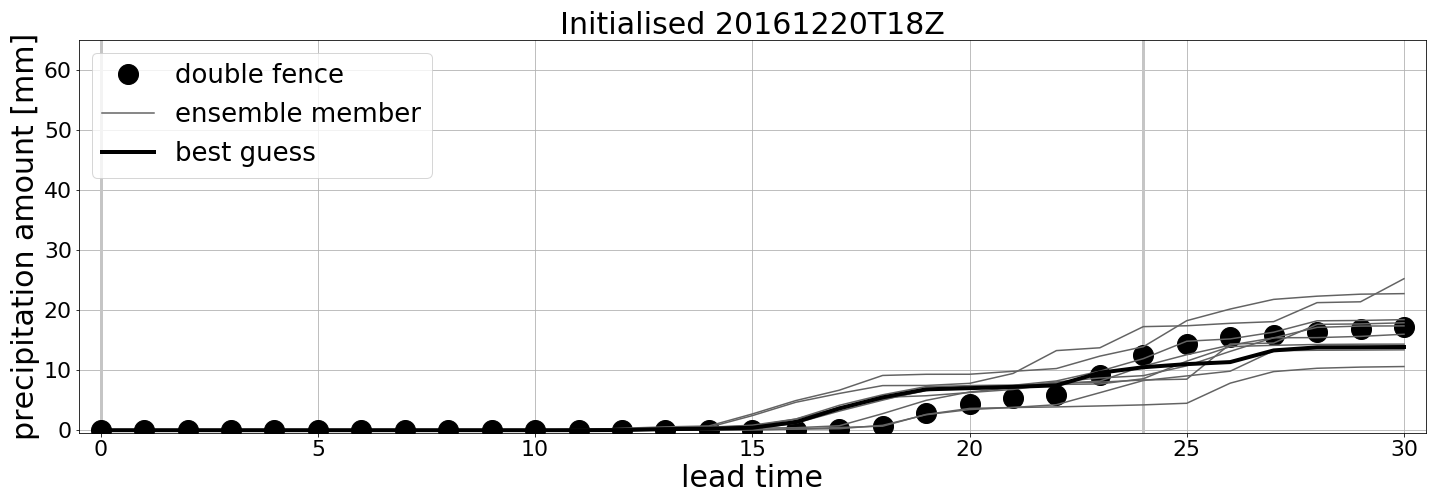
\includegraphics[
        width=\textwidth]{./fig_MEPS_sfc/20161220_18}
        \caption{}\label{fig:acc20}
        %\label{fig:DT2100}
    \end{subfigure}
    \hfill
%%%%%% 21/12
    \begin{subfigure}[b]{0.49\textwidth}
        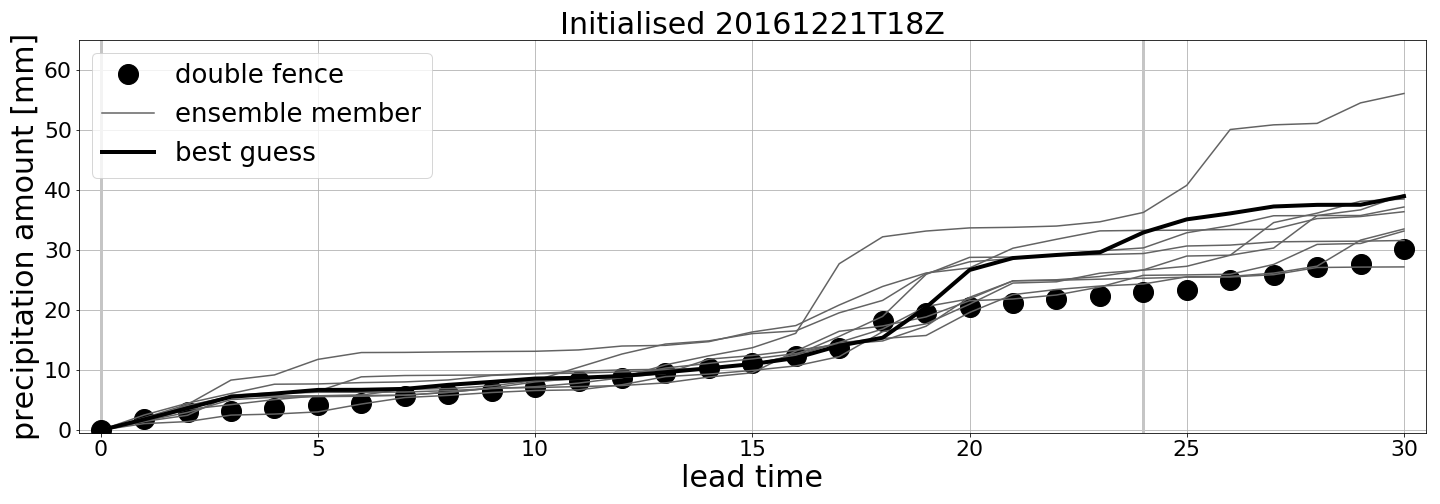
\includegraphics[
        width=\textwidth]{./fig_MEPS_sfc/20161221_18}
        \caption{}\label{fig:acc21}
    \end{subfigure}
%%%%%% 22/12
    \begin{subfigure}[b]{0.49\textwidth}
        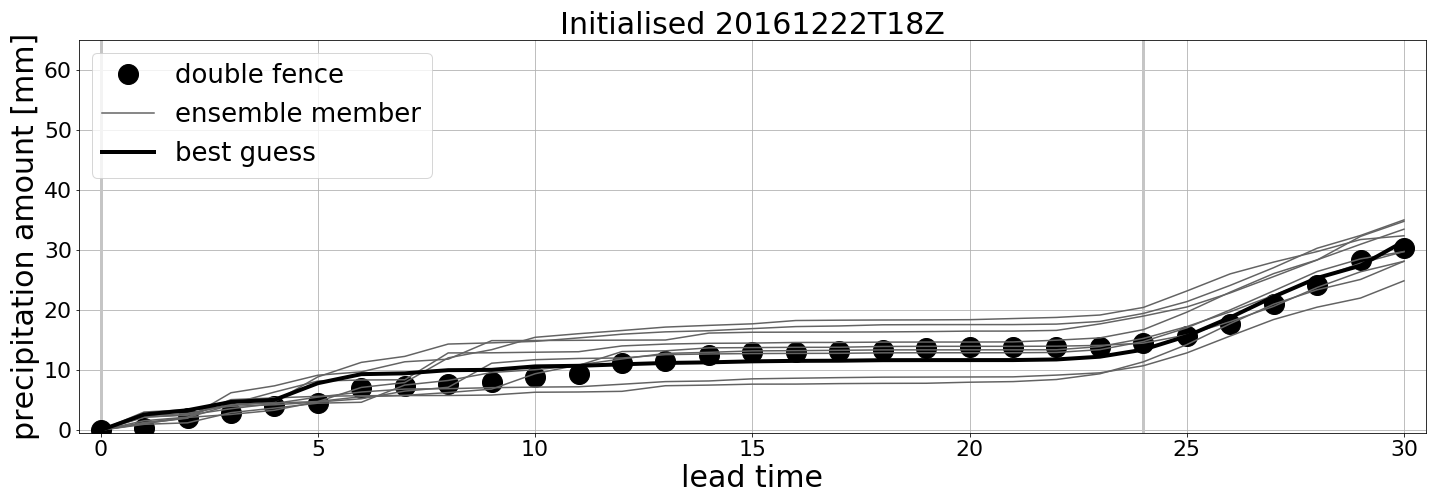
\includegraphics[
        width=\textwidth]{./fig_MEPS_sfc/20161222_18}
        \caption{}\label{fig:acc22}
    \end{subfigure}
    \hfill
%%%%%% 23/12
    \begin{subfigure}[b]{0.49\textwidth}
        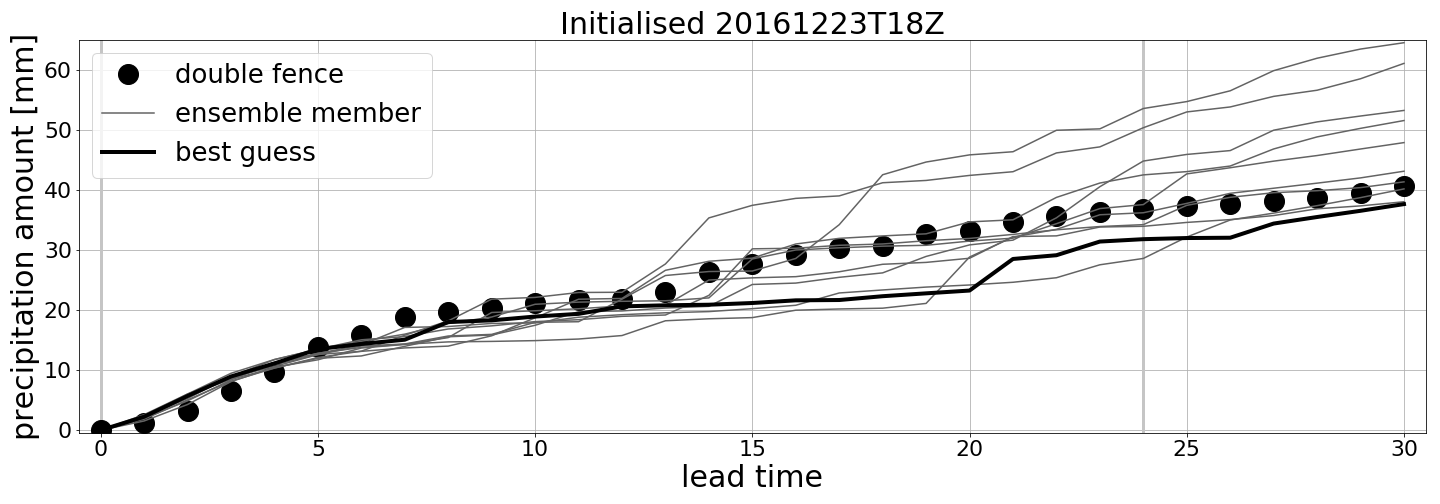
\includegraphics[
        width=\textwidth]{./fig_MEPS_sfc/20161223_18}
        \caption{}\label{fig:acc23}
    \end{subfigure}
%%%%%% 24/12
    \begin{subfigure}[b]{0.49\textwidth}
        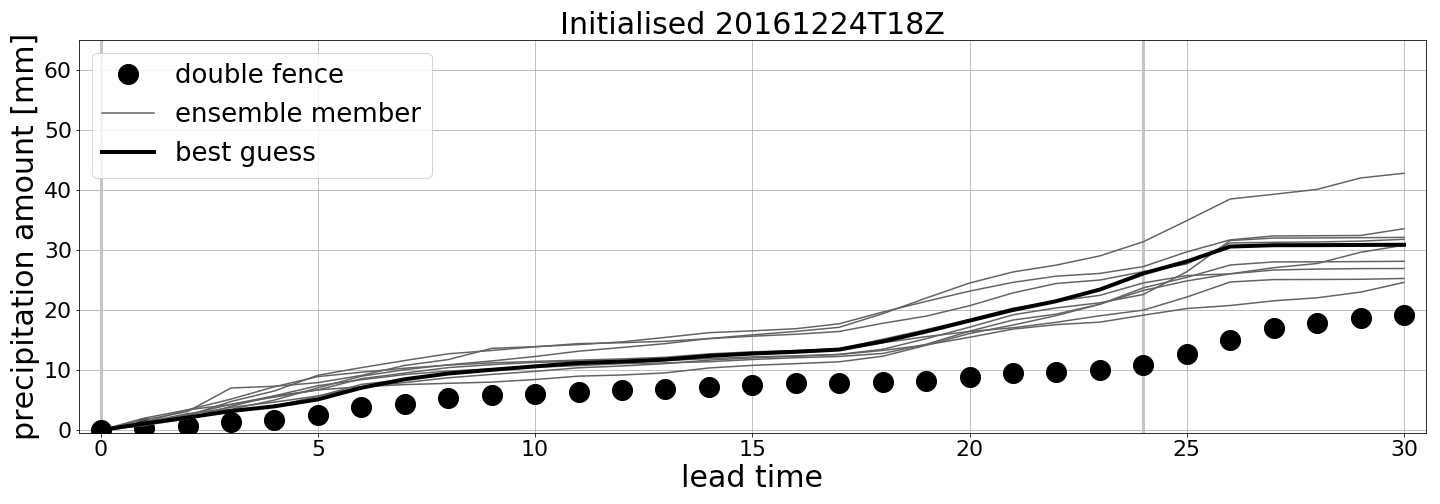
\includegraphics[
        width=\textwidth]{./fig_MEPS_sfc/20161224_18}
        \caption{}\label{fig:acc24}
    \end{subfigure}
    \hfill
%%%%%% 25/12
    \begin{subfigure}[b]{0.49\textwidth}
        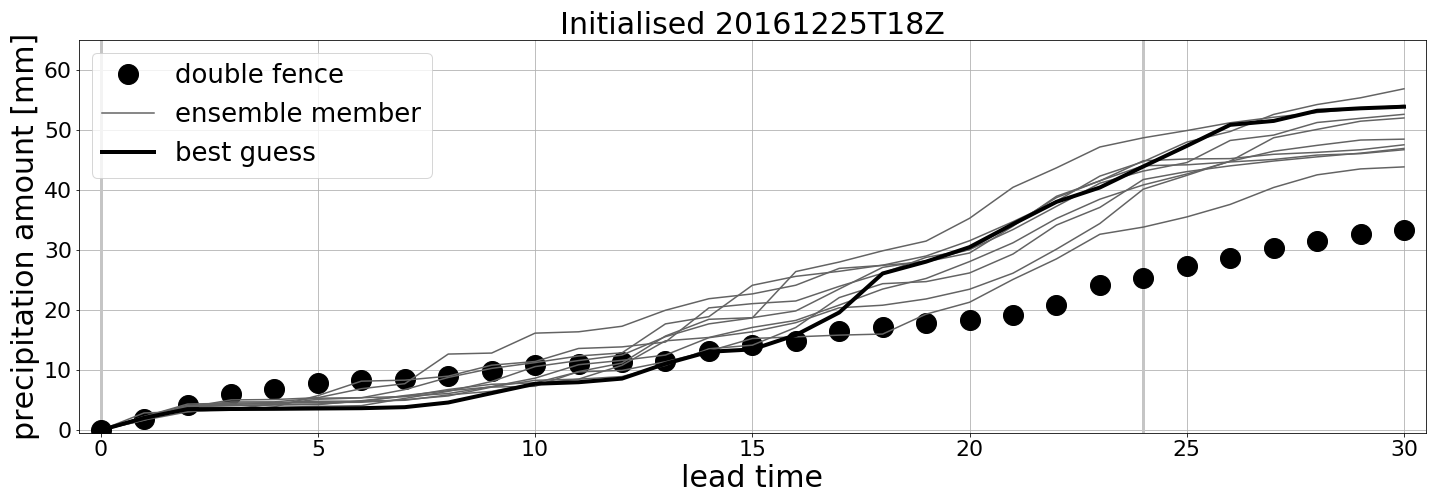
\includegraphics[
        width=\textwidth]{./fig_MEPS_sfc/20161225_18}
        \caption{}\label{fig:acc25}
    \end{subfigure}
    \caption{Accumulation of precipitation at Haukeliseter. Initalisation of MEPS at \SI{18}{\UTC}. Ensemble member as line in grey and the control in black. Dots indicate the hourly accumulation observed at the double fence, \citep{eklima_norwegian_2016}. \textcolor{red}{Do you think I have to make something bigger??? Font size etc? Or use one page only for the figures and have them underneath each other?} } \label{fig:acc20_25}
\end{figure}
%%%%%%%%%%%%%%%%%%%%%%%%%%%%%%%%%%%%%%%%%%%%%%%%%%%%%%%%%%%%%%%%%%%%%%%%%%
\noindent
During Christmas 2016 a storm approached the Haukeliseter site, which resulted in precipitation in form of liquid and solid.
\Cref{fig:acc20_25} shows the preliminary comparison between the MEPS ensemble member forecasts as well as the snowfall accumulation measured by the double fence at Haukeliseter. The double fence data is noisy and therefore, a filtered dataset is accessed from \cite{eklima_norwegian_2016}.   
\\
Each MEPS cycle is initialized at \SI{18}{\UTC} for the respective day.
Grey lines in \Cref{fig:acc20_25} show the nine perturbed ensemble members of MEPS. Where the black line reflects the control run, and the dots accumulation by the double fence.
\\
During the first few days the ensemble outputs cover the amount of snow good in comparison to the double fence observations.
The spread of the ensemble members around the control run fits as well to the observations for this time period. But, for an initialisation on the \SI{24}{\dec}, \SI{18}{\UTC} one can see that  MEPS over estimates the amount of snow accumulation. It is even more pronounced with the initialisation on the \SI{25}{\dec}, \SI{18}{\UTC} (compare \Cref{fig:acc25}). 
\\
This can have different reasons. One of them can be that the large scale weather situation was more predictable for the first four days (\Cref{fig:acc20,fig:acc21,fig:acc22,fig:acc23}). 
According to \cite{muller_arome-metcoop:_2017} are strong precipitation events better predicted with MEPS than ECMWF (European Centre for Medium-Range Weather Forecasts). On the other side, \cite{muller_arome-metcoop:_2017} states, that an overestimation appears, where the precipitation event (\SI{12}{\hour} accumulation) is less than \SI{10}{\mm}. This is not the case for the time period \SIrange{21}{26}{\dec} (compare \Cref{fig:DecObs}), where the daily precipitation exceed \SI{10}{\mm} every day. The question arises why MEPS covers the high amount of snow accumulation on the \SI{24}{\dec} but forecasts \SI{24}{\hour} prior to \SIlist{25;26}{\dec} are not covering the predicted amount of accumulation!